\section{Introduction}
Imagine a robot reaching for an object after its motors have become weaker.
The same command now produces a different movement. A world model can detect
this discrepancy: it predicts the outcome of a command, observes the actual
outcome, and measures the difference. The question is how to use that new
experience. Updating the model is one option. Another is to keep the trained
model intact and learn a small correction alongside it.

This second option is useful when a representation serves several purposes.
A model may predict future observations, recognize semantic categories, and
associate information across sensors. Deployment feedback about an actuator
provides a direct signal for dynamics prediction, while the model's other
outputs may need to remain stable. A separate correction can learn from this feedback while the trained
representation remains fixed.

World models learn representations through prediction
\citep{ha2018worldmodels,hafner2019planet,hafner2020dreamer}.
For a sequence predictor, the timing and order of observations can matter as
much as their content. We choose a spiking temporal core to make recent input
history part of the computation: membrane variables accumulate incoming signals,
leak over time, and emit spikes when their accumulated value crosses a threshold.
This gives the model a mechanism for representing temporal patterns, which
surrogate-gradient training can learn to use \citep{yu2026beyondrate}.
Causal attention combines these signals using only the observed prefix.
Our controlled event-model probes support this temporal motivation: future
prediction is more accurate with ordered sequences than when event features
are shuffled or sorted onto a regular time grid
(Section~\ref{sec:temporal_evidence}).

Audio, visual features, rendered words, and state--action inputs enter through
appropriate adapters. Each adapter preserves its stream's prediction target; all streams use the
same temporal core. We use \emph{next-spike prediction} to describe this
event-oriented learning approach and specify the actual next-feature and
action-outcome targets in Section~\ref{sec:model}.

\begin{figure}[tbp]
\centering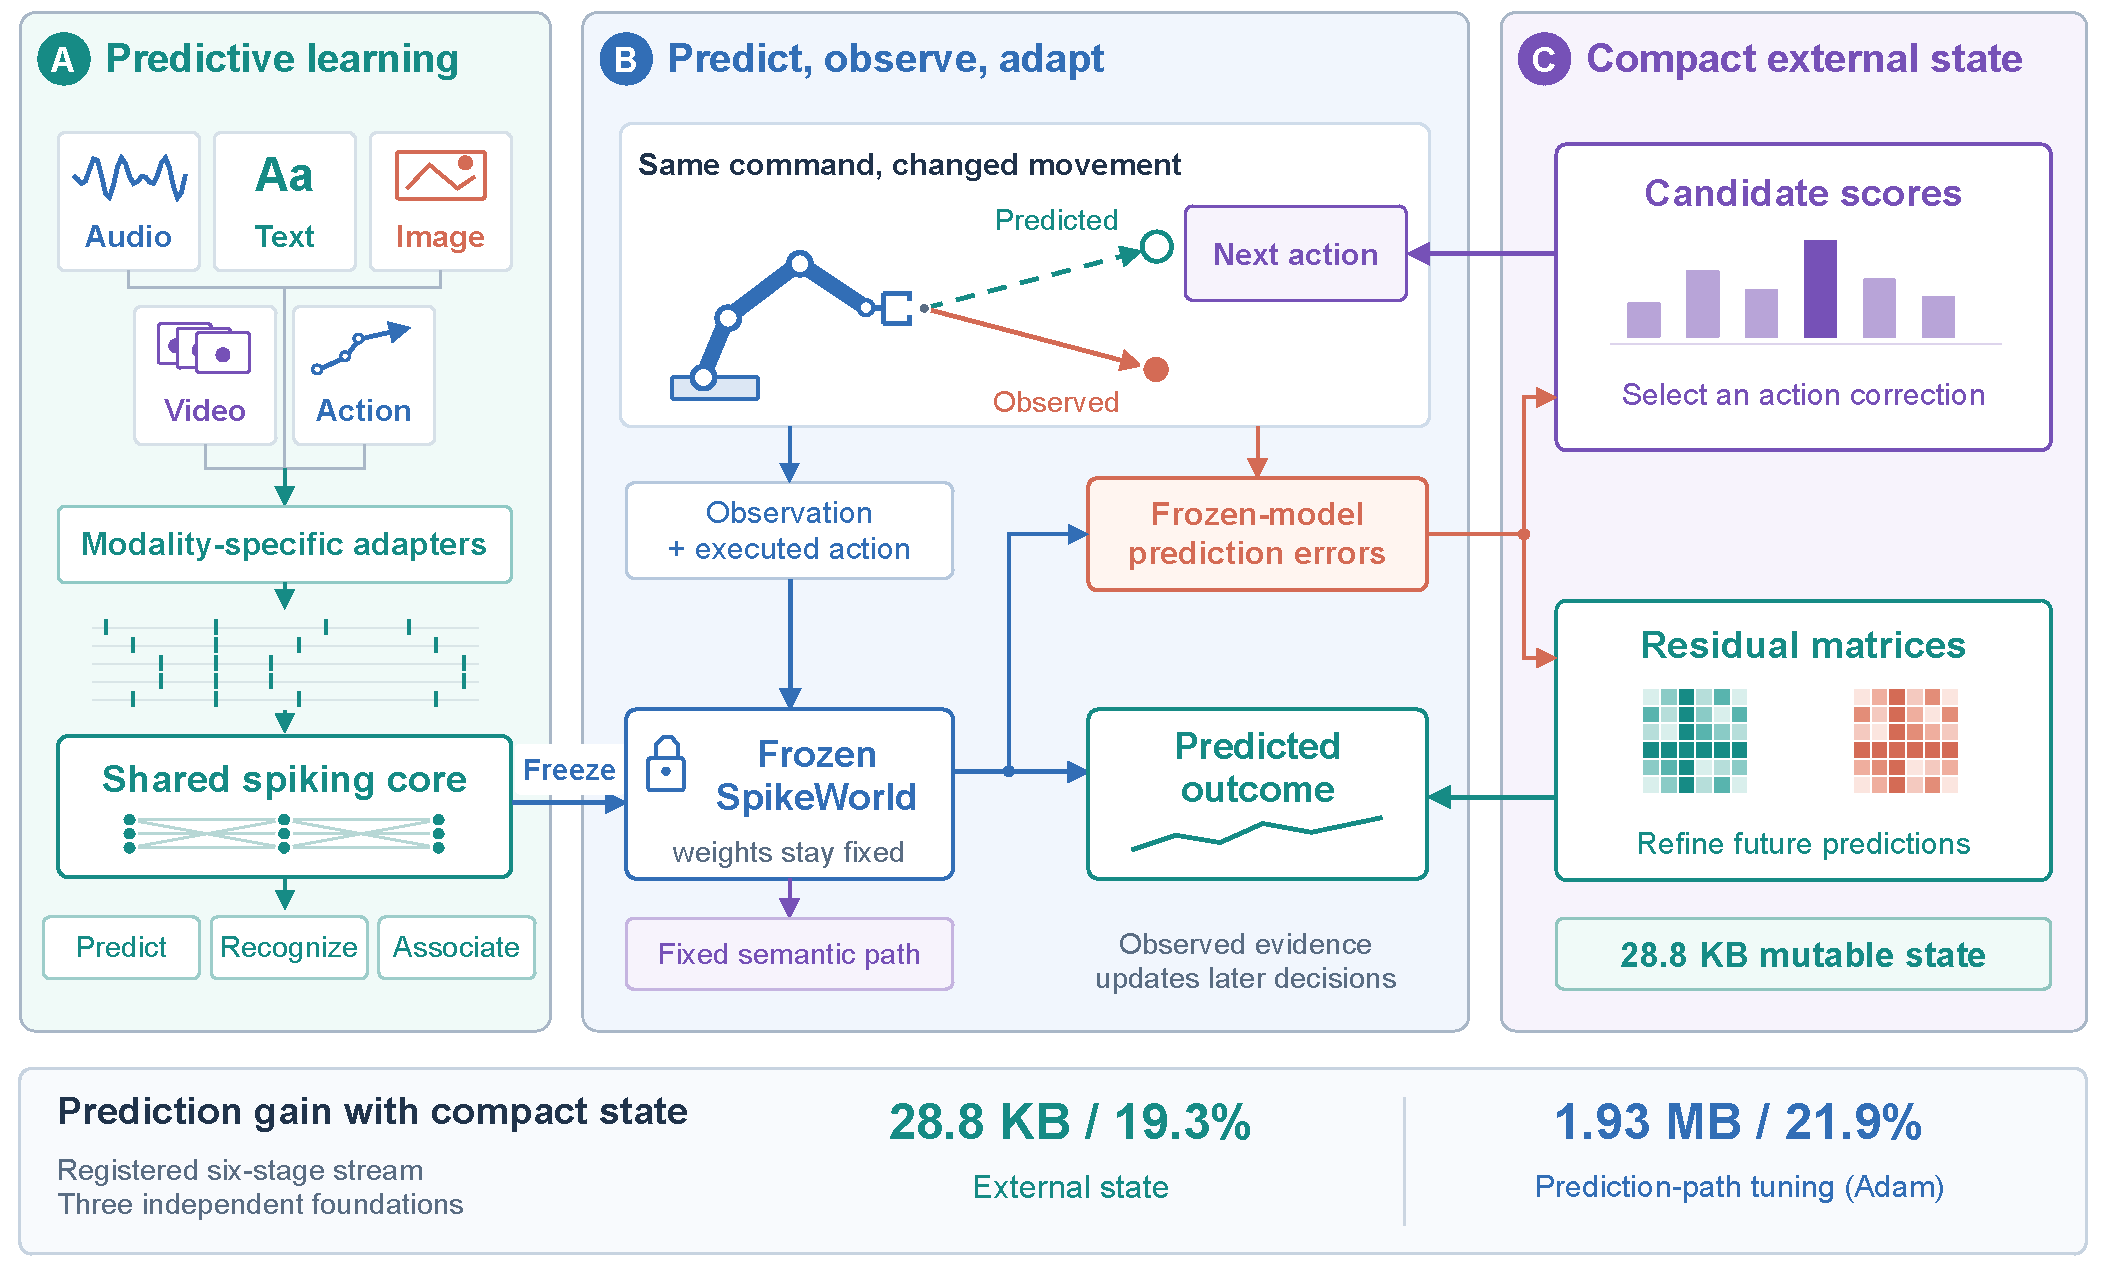
\includegraphics[width=\linewidth]{fig1_workflow.pdf}
\caption{\textbf{A shared predictive model, with room to learn outside its weights.}
\textbf{A}, sensory and action inputs enter through modality-specific adapters
and train a shared spiking core for prediction, recognition, and association.
\textbf{B}, the selected checkpoint is frozen. The robot illustration shows
how changed actuation creates a difference between expected and observed movement.
Outcomes evaluated through the frozen predictor supply online learning evidence.
\textbf{C}, candidate scores select a bounded correction to a later command
(purple); residual matrices refine the prediction (teal). The semantic path
retains its fixed-input mapping. The bottom strip summarizes the main-stream
prediction--storage comparison. Icons, trajectories, scores, and matrix patterns
are schematic; the bottom-strip values are measured results.}
\label{fig:workflow}
\end{figure}

Figure~\ref{fig:workflow} connects this learning process to deployment.
The left panel gathers heterogeneous inputs into a shared predictive model.
The center panel returns to the weakened-motor example: the selected model
stays fixed while newly observed outcomes provide evidence about the change.
The predictor trained offline thus supplies the error signal for online learning.
The right panel shows where that experience is stored. Residual matrices
correct hidden features for prediction, while a separate score vector compares
registered actuator transformations and chooses a bounded command correction.
An existing control policy proposes the command; this interface adjusts it
to compensate for the identified actuator change.
The colored paths show how each correction is used. We can disable either
component to test its effect on prediction and commands.

We find that a small external state recovers most of the prediction improvement
of the evaluated prediction-path fine-tuning configuration. This comparison
uses a six-stage stream containing source, attenuation, and shear conditions
and measures how much mutable state each method requires. Component interventions show that the matrices account for additional
prediction accuracy, while the score-and-inverse path accounts for changed
commands. A separate closed-loop experiment connects the latter to reward.

We make three contributions. We train and evaluate a shared predictive--semantic
spiking model with sensory and action targets. We design an online interface
that stores corrections in bounded external state and preserves the trained
semantic mapping. We measure its prediction--storage trade-off and test the
separate roles of its state components. The appendix provides the full equations,
protocols, additional comparisons, and code-to-result map. Code, editable figures,
and recorded experiment outputs are available at
\url{https://github.com/Oooorca/SpikeWorld}.
